\documentclass{beamer}
\usepackage{ hyperref}
\usepackage[T1]{fontenc}
\usepackage{algorithm,algorithmic}
\renewcommand{\algorithmicrequire}{\textbf{Input:}}  % Use Input in the format of Algorithm  
\renewcommand{\algorithmicensure}{\textbf{Output:}} % Use Output in the format of Algorithm  


% \usepackage[orientation=landscape,size=custom,width=16,height=9,scale=0.4,debug]{beamerposter}
% 修改 slides 比例,

% other packages
\usepackage{latexsym,amsmath,xcolor,multicol,booktabs,calligra}
\usepackage{graphicx,pstricks,listings,stackengine,cite}
\usetheme{Berkeley}
\setbeamertemplate{bibliography item}[text]
\bibliographystyle{plain}
\author{Xiuqi Zhang \quad Zikun Zhou\quad Heyin Shen \quad Anna Lee}
\title{Project 1 \\Lattice-based Cryptography}
\institute{JI SJTU}
\date{\today}
\lstset{
	basicstyle=\ttfamily\small,
	keywordstyle=\bfseries\color{deepblue},
	emphstyle=\ttfamily\color{deepred},    % Custom highlighting style
	stringstyle=\color{deepgreen},
	numbers=left,
	numberstyle=\small\color{halfgray},
	rulesepcolor=\color{red!20!green!20!blue!20},
	frame=shadowbox,
}


\begin{document}
	\begin{frame}
		\titlepage
	\end{frame}

	\begin{frame}
		\tableofcontents
	\end{frame}

	\section{Introduction}
	\begin{frame}
		\begin{itemize}
			\item Lattice-based cryptography is a general set of cryptography that involves lattices.
			\item Lattice-based cryptosystems covers encryption, signatures and hash functions.
			\item Lattice-based cryptosystems are (still) post-quantum computing se- cure, and have proved security basing on worst-case scenario.
		\end{itemize}
	\end{frame}
	
	\section{Lattice}
	\begin{frame}{Introduction of Lattice}
		Less formally (while not indicating less accurate), lattice can be viewed as a set of points
		\begin{equation}
			L=\{a_1v_1+a_2v_2+...+a_nv_n|a_i\in\mathbb{Z}\}
		\end{equation}
		$(v_1,v_2,...,v_n)\in\mathbb{R}^n$ and they are linear independent
		
	\end{frame}
	\begin{frame}{Example}
		% we integra figure 1
		All points forming the lattice can be generated by linear combination with integer coefficients. We denote the set $B = \{v1,v2,...,vn\}$ as basis of the latice. Then the lattice can also be denoted as $L(B)$. Apparently basis is not unique.
	\end{frame}
	\subsection{Equivalent Bases}
	\subsubsection{Column View}
	\begin{frame}{Column View}
		\begin{itemize}
			\item Changing order of $\forall v_i,v_j\in B$ does not chagne the lattice generated.
			\item $\forall v_i\in B, L(B')=L(B)$ where $B'=(B/v_i)\cup \{-v_i\}$.
			\item Linear Combination: for some $v_i, v_j\in B$, let $v_i=v_i+kv_j$ where $k\in \mathbb{Z}$.
		\end{itemize}
	\end{frame}
	
	\subsubsection{Matrix View}
	\begin{frame}{Theorem}
		\begin{theorem}
			\begin{equation}
				L(B_1)=L(B_2) \iff B_1=B_2U
			\end{equation}
			where $U$ is a unimodular $U$.
		\end{theorem}
	\end{frame}
	
	\subsection{Lattice meaning to space}
	\begin{frame}
		% this  to interprete figure 2
	\end{frame}
	
	\begin{frame}
		Notice that no matter which basis is chosen, the fundamental parallelpiped has the same volume. This can be proved by imagining a very large space where the shape of each small region can be ignored. Since the number of small regions is the same the volumn of them should be the same.
		
		We define the determinant of a lattice $L(B)$ as  $\det(L)=|\det(B)|$, which is the volume of the fundomental parallelepiped.
	\end{frame}
	\subsection{Successive Minima}
	\begin{frame}{Successive Minima}
		One very important element of a lattice is the shortest vector in the lattice. We denote the length (Euclidean norm) of the shortest vectors in $\mathcal{L}$ as $\lambda_1(\mathcal{L})$, the second shortests as $\lambda_2(\mathcal{L})$,\ldots, etc. 
	\end{frame}
	\subsection{Gram-Schmidt Orthogonalization}
	\begin{frame}{Gram-Schmidt Orthogonalization}
		Gram-Schmidt Orthogonalization is a process which takes a set of linearly inde- pendent vectors and output a set of orthogonal vectors with same cardinality. It projects each vector on the orthogonal complement of the previous vectors. A formal design is as Eq.~\ref{eq:gso}
		
		For vector series $B=b_{1}, b_{2}, \ldots, b_{n}$, GSO vector set $\widetilde B=\tilde{b}_{1}, \tilde{b}_{2}, \ldots, \tilde{b}_{n}$ is as
		
		\begin{equation}
			\label{eq:gso}
			\tilde{b}_{i}=b_{i}-\sum_{j=1}^{i-1} \mu_{i, j} \tilde{b}_{j}, \text { where } \mu_{i, j}=\frac{\left\langle b_{i}, \tilde{b}_{j}\right\rangle}{\left\langle\tilde{b}_{j}, \tilde{b}_{j}\right\rangle}
		\end{equation}
	\end{frame}
	\subsection{Minkowski's Theorem}
	\begin{frame}{Minkowski's Theorem}
		\begin{theorem}
			\label{thm:minkowski}
			\textbf{Minkowski's Theorem:} For any lattice $\Lambda$ and convex zero-symmetric set $S$, volume of which is larger than $2^n\det(\Lambda)$, there must exists some lattice point in $S$. (which is the upper bound of smallest lattice).
		\end{theorem}
		\begin{theorem}
			\textbf{Inference of Minkowski's Theorem:}
			\begin{equation}
				\forall \Lambda, \lambda_1(\Lambda)\leq \sqrt{n}\cdot \det(\Lambda)^ {\frac{1}{n} }
			\end{equation}
		\end{theorem}
	\end{frame}
	\section{Basic Computation Lattice Problems}
	\subsection{Shortest Vector Problem (SVP)}
	\begin{frame}
		Shortest\footnote{If not specified, all discussion about length in this report is Euclidean norm.} Vector Problem is the most important and basic computation problem about lattice. From Theorem~\ref{thm:minkowski} and Theroem~\ref{thm:lower_bound_lattice} we know about the upper and lower bound of shortest vector, however it does not provide a way to find such vector. This problems remains to be a hard problem, and works in the field of lattice compuatation problems as basic as SAT problem in NP-complete.
	\end{frame}
	\subsubsection{Hardness}%
	\begin{frame}{Hardness}
			In Euclidean distance, which as most scenario this report is discussed on, we only know that by applying randomized reductions the problem is NP-hard~\cite{SVP_random}. If considering uniform norm, the problem has already been proved to be NP-hard~\cite{SVP_exact}.
	\end{frame}

	\subsubsection{GapSVP}%
	\begin{frame}{GapSVP}
		GapSVP$_\gamma$ is variant of SVP$_\gamma$, in which we try to know that whether $\lambda(\mathcal{L}(B))$ is not bigger than one, or larger than $\gamma$, where $\gamma$ is some function $f(n)$, where $n$ is the dimension of the space. Notice that it is a promise problem, which means input should make sure the result will in one of the conditions.
	\end{frame}
	\subsection{Closest vector problem (CVP)}%
	\begin{frame}
		The closest vector problem is about in following scenario:
		
		A basis $B$ and a lattice $L$, and some vector $v\in \vec(B)$.
		
		Try to find:
		
		A vector $v'\in L$, which is closest to $v$.
	\end{frame}
	
	\subsubsection{Hardness}
	\begin{frame}{Hardness}
		urther from the conclusion that we can solve SVP efficiently if we can solve CVP, Goldreich et al.\ proved that CVP is at least harder than SVP at any aspect~\cite{RN3}. Dinur et al. proved that, with factor $n^{c/\log{\log{n}}}$ for some constant $c>0$, CVP is NP-hard to approximate~\cite{GMSS99}.
	\end{frame}
	\subsubsection{Summary}
	In summary, the hardness about the problem (currently) according to factor is as Figure
	% Here Figure 3
	\section{Advantage of Lattice-based cryptography}
	\begin{frame}{Anti-quantum Attack}
		This is the main advantage the lattice-based cryptography has over the traditional public-key cryptographies as the security of the latter has been challenged in the context of a quantum computer. In fact, the security guarantee of most traditional public-key cryptographies is established based on the hardness of the factorization of large integers, the discrete logarithm and other related problems. However, with the proposition of the quantum algorithm, both factoring and discrete algorithm-based problems are solvable in polynomial time complexity. Therefore, in the research of modern public-key cryptosystem, lattice-based cryptography outstands for its ability to resist quantum attacks.
	\end{frame}
	\subsection{Efficient algorithm and high concurrency} 
	\begin{frame}
		The main mains problems involved in the lattice-based cryptosystem are based on the calculation of vectors without the engagement of large prime integers, and the algorithm also enjoys relative high concurrency, leading to high efficiency in practice.
	\end{frame}
	\subsection{Worst case to average case reduction}
	\begin{frame}
		The security of the lattice-based cryptography can be guaranteed because it is built based on the "worst case to average case reduction". In other words, the hardness of finding the solutions of a certain problems in average cases is no less than finding the solutions in the worst cases. In practice, efficient lattice-based algorithms, such as those that are based on LWE, their worst-case hardness results may be unknown. Conversely, cryptographic that are based on factoring, which we know is hard in the worst case, can still be decrypted easily when it is easy to solve the factorization on average input. While as lattice-based cryptosystem is hard to solve in the worst case, it possesses very high security.
	\end{frame}
	\section{Shortest Integer Solution Problem (SIS)}
	\begin{frame}{Introduction}
		The short integer solution problem (SIS) is an average-case problem based on the worst-case lattice problem. Its difficulty is guaranteed by the short vector problem
	\end{frame}
	\subsection{Definition}
	\begin{frame}{Definition}
		There is a relationship between the SIS and the lattice problems:\\
		Let $S$ be the set of all solution $\mathbf{z}$, such that $\mathbf{A}\mathbf{z}=0\pmod{q}$. As this set is additive, $S$ is a lattice. Therefore, the SIS problem can be regarded as the problem to find a short vector in $S$.\\
		Now we have a new representation of lattices constructed from matrix $\mathbf{A}$:
		\begin{equation}
			L^{\perp}(\mathbf{A})=\{\mathbf{z}\in\mathbb{Z}^m: \mathbf{A}\mathbf{z}=0 \pmod{q}\}
		\end{equation}
		Using worst-case to average-case reduction, solving the SIS problem in $L^{\perp}(\mathbf{A})$ is approximately solving SVP in all lattices, which will be discussed later.
	\end{frame}
	\subsection{One-Way \& Collision-Resistant Hash Function using SIS}
	\begin{frame}{Hash Function}
		An one-way \& collision-resistant hash function can be easily implied from the SIS:\\
		Set $m>n\lg{q}$. Given random $\mathbf{A}$ in $\mathbb{Z}^{n\times m}_q$, define the hash function $f_{\mathbf{A}}:\{0,1\}^m\rightarrow \mathbb{Z}^n_q$ as:
		\begin{equation}
			f_{\mathbf{A}}(\mathbf{z})=\mathbf{A}\mathbf{z}
		\end{equation}
		A collision $f_{\mathbf{A}}(\mathbf{z})=f_{\mathbf{A}}(\mathbf{y})$ yields a solution $\mathbf{z}-\mathbf{y}$ of SIS for $\mathbf{A}$, as $\mathbf{z}-\mathbf{y}$ is in $\{0,1\}^m$ and satisfy $\mathbf{A}(\mathbf{z}-\mathbf{y})=0$
	\end{frame}
	\subsection{Worst-case to Average-case Reduction}
	\subsubsection{Uniform Distribution Over Lattices}
	\begin{frame}
		\begin{theorem}
			If $s>5\lambda_n(\mathbf{B})$, and $\mathbf{X}\sim \rho_s(\mathbf{x})=(1/s)^ne^{-\pi ||\mathbf{x}||^2/s^2}$, then
			
			\begin{equation}
				\Delta(\mathbf{X}\mod{\mathbf{B}},\mathrm{Uniform }(\mathbf{B}))<n2^{-110}
			\end{equation}
			\label{thm:uniform_distribution}
		\end{theorem}
	\end{frame}
	\begin{frame}
		\begin{figure}[H]
			\centering
			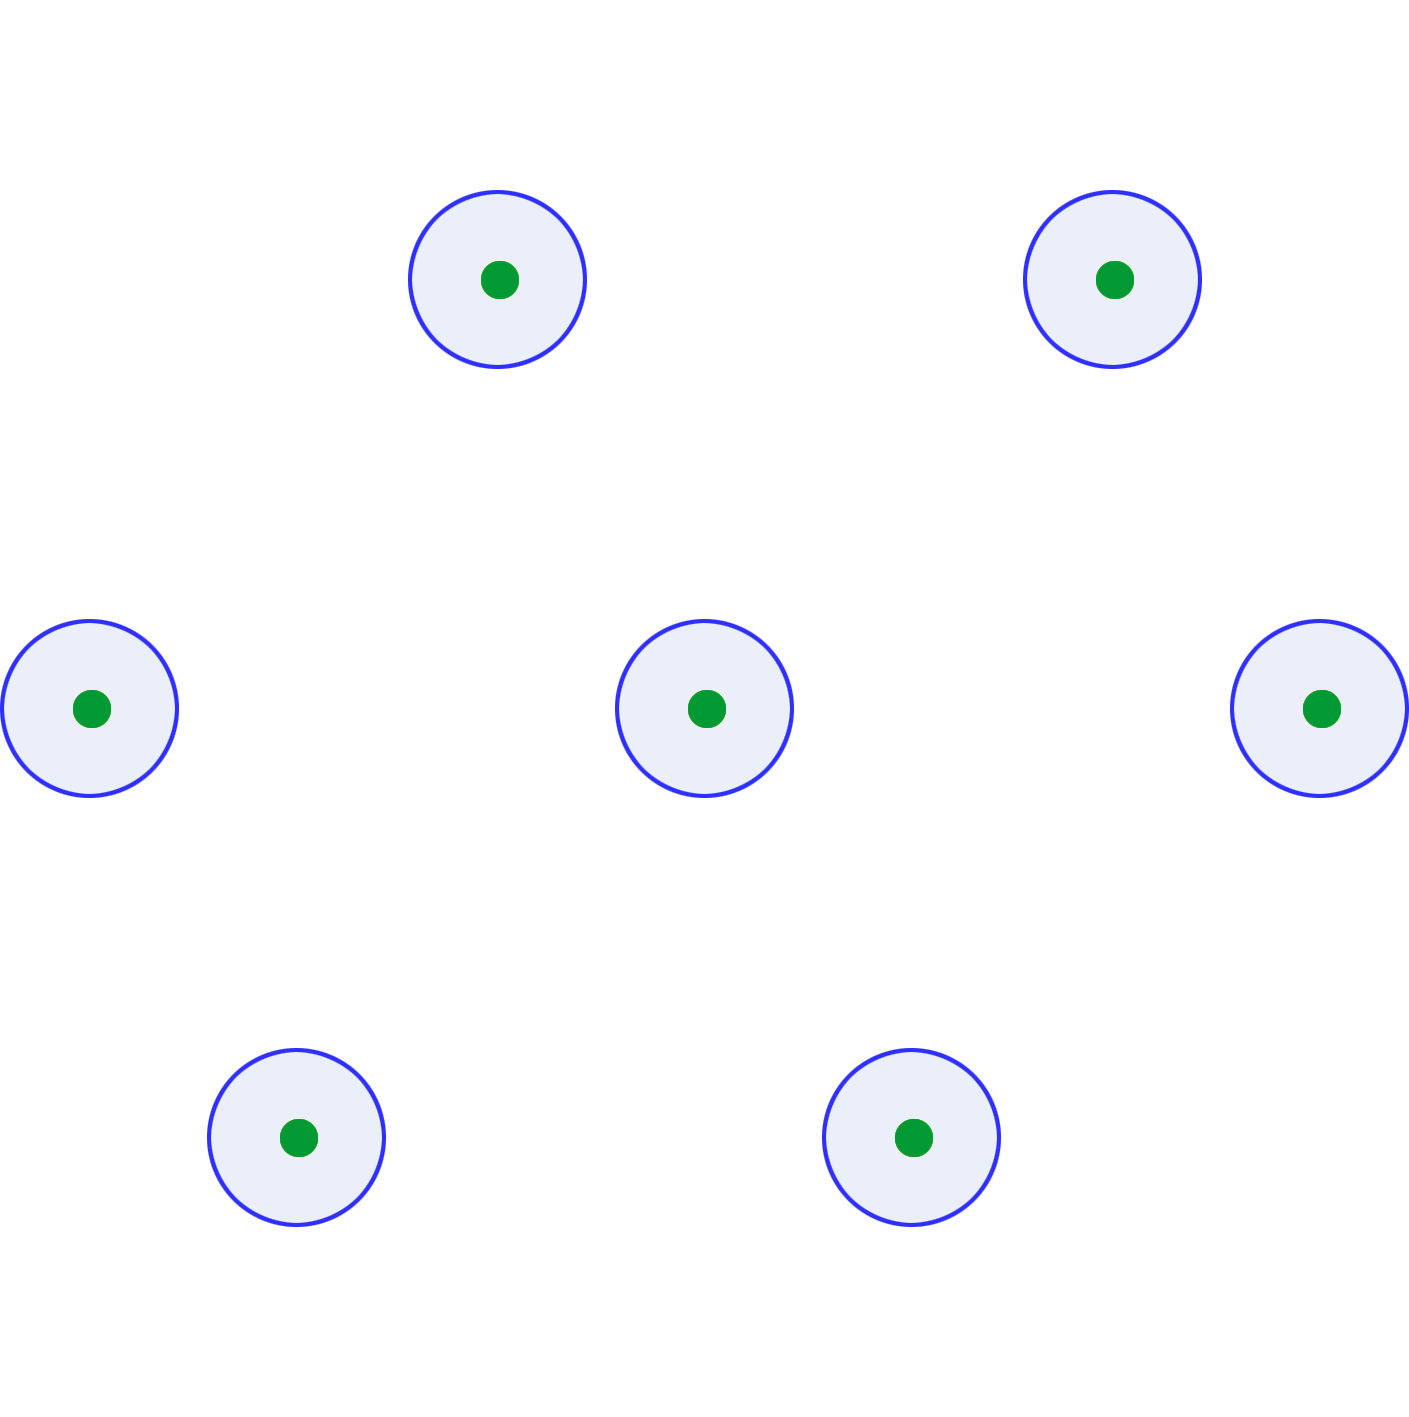
\includegraphics[width=0.5\linewidth]{./image/gaussian_1.png}
			\caption{The distribution when $s$ is small}%
			\label{fig:gaussian_1}
		\end{figure}
	\end{frame}
	\begin{frame}
		\begin{figure}[H]
		\centering
		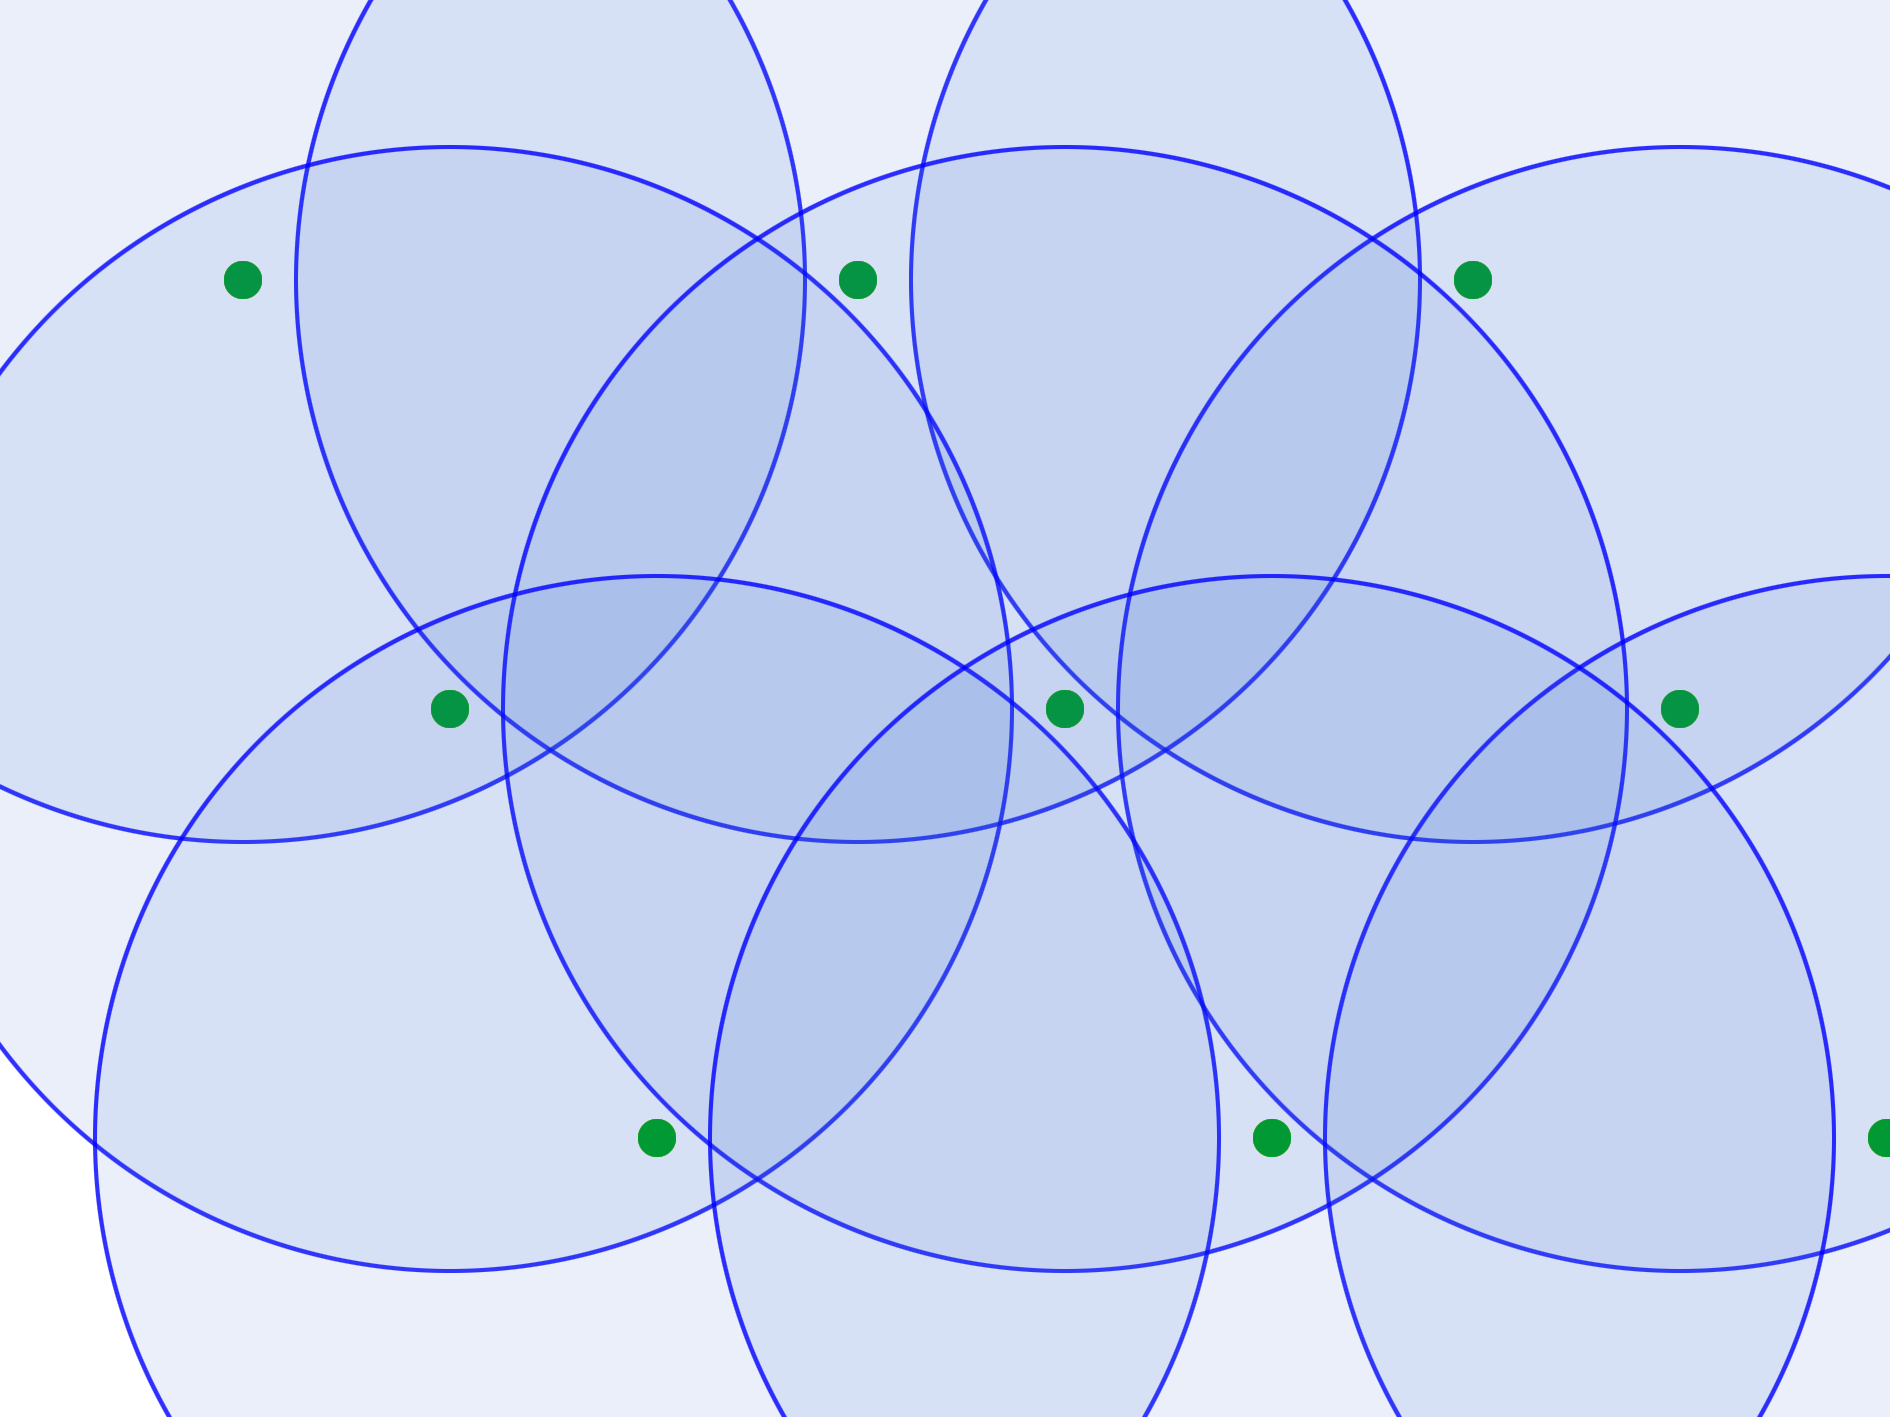
\includegraphics[width=0.5\linewidth]{./image/gaussian_2.png}
		\caption{The distribution when $s$ increases}%
		\label{fig:gaussian_2}
		\end{figure}
	\end{frame}
	\begin{frame}
		\begin{figure}[H]
			\centering
			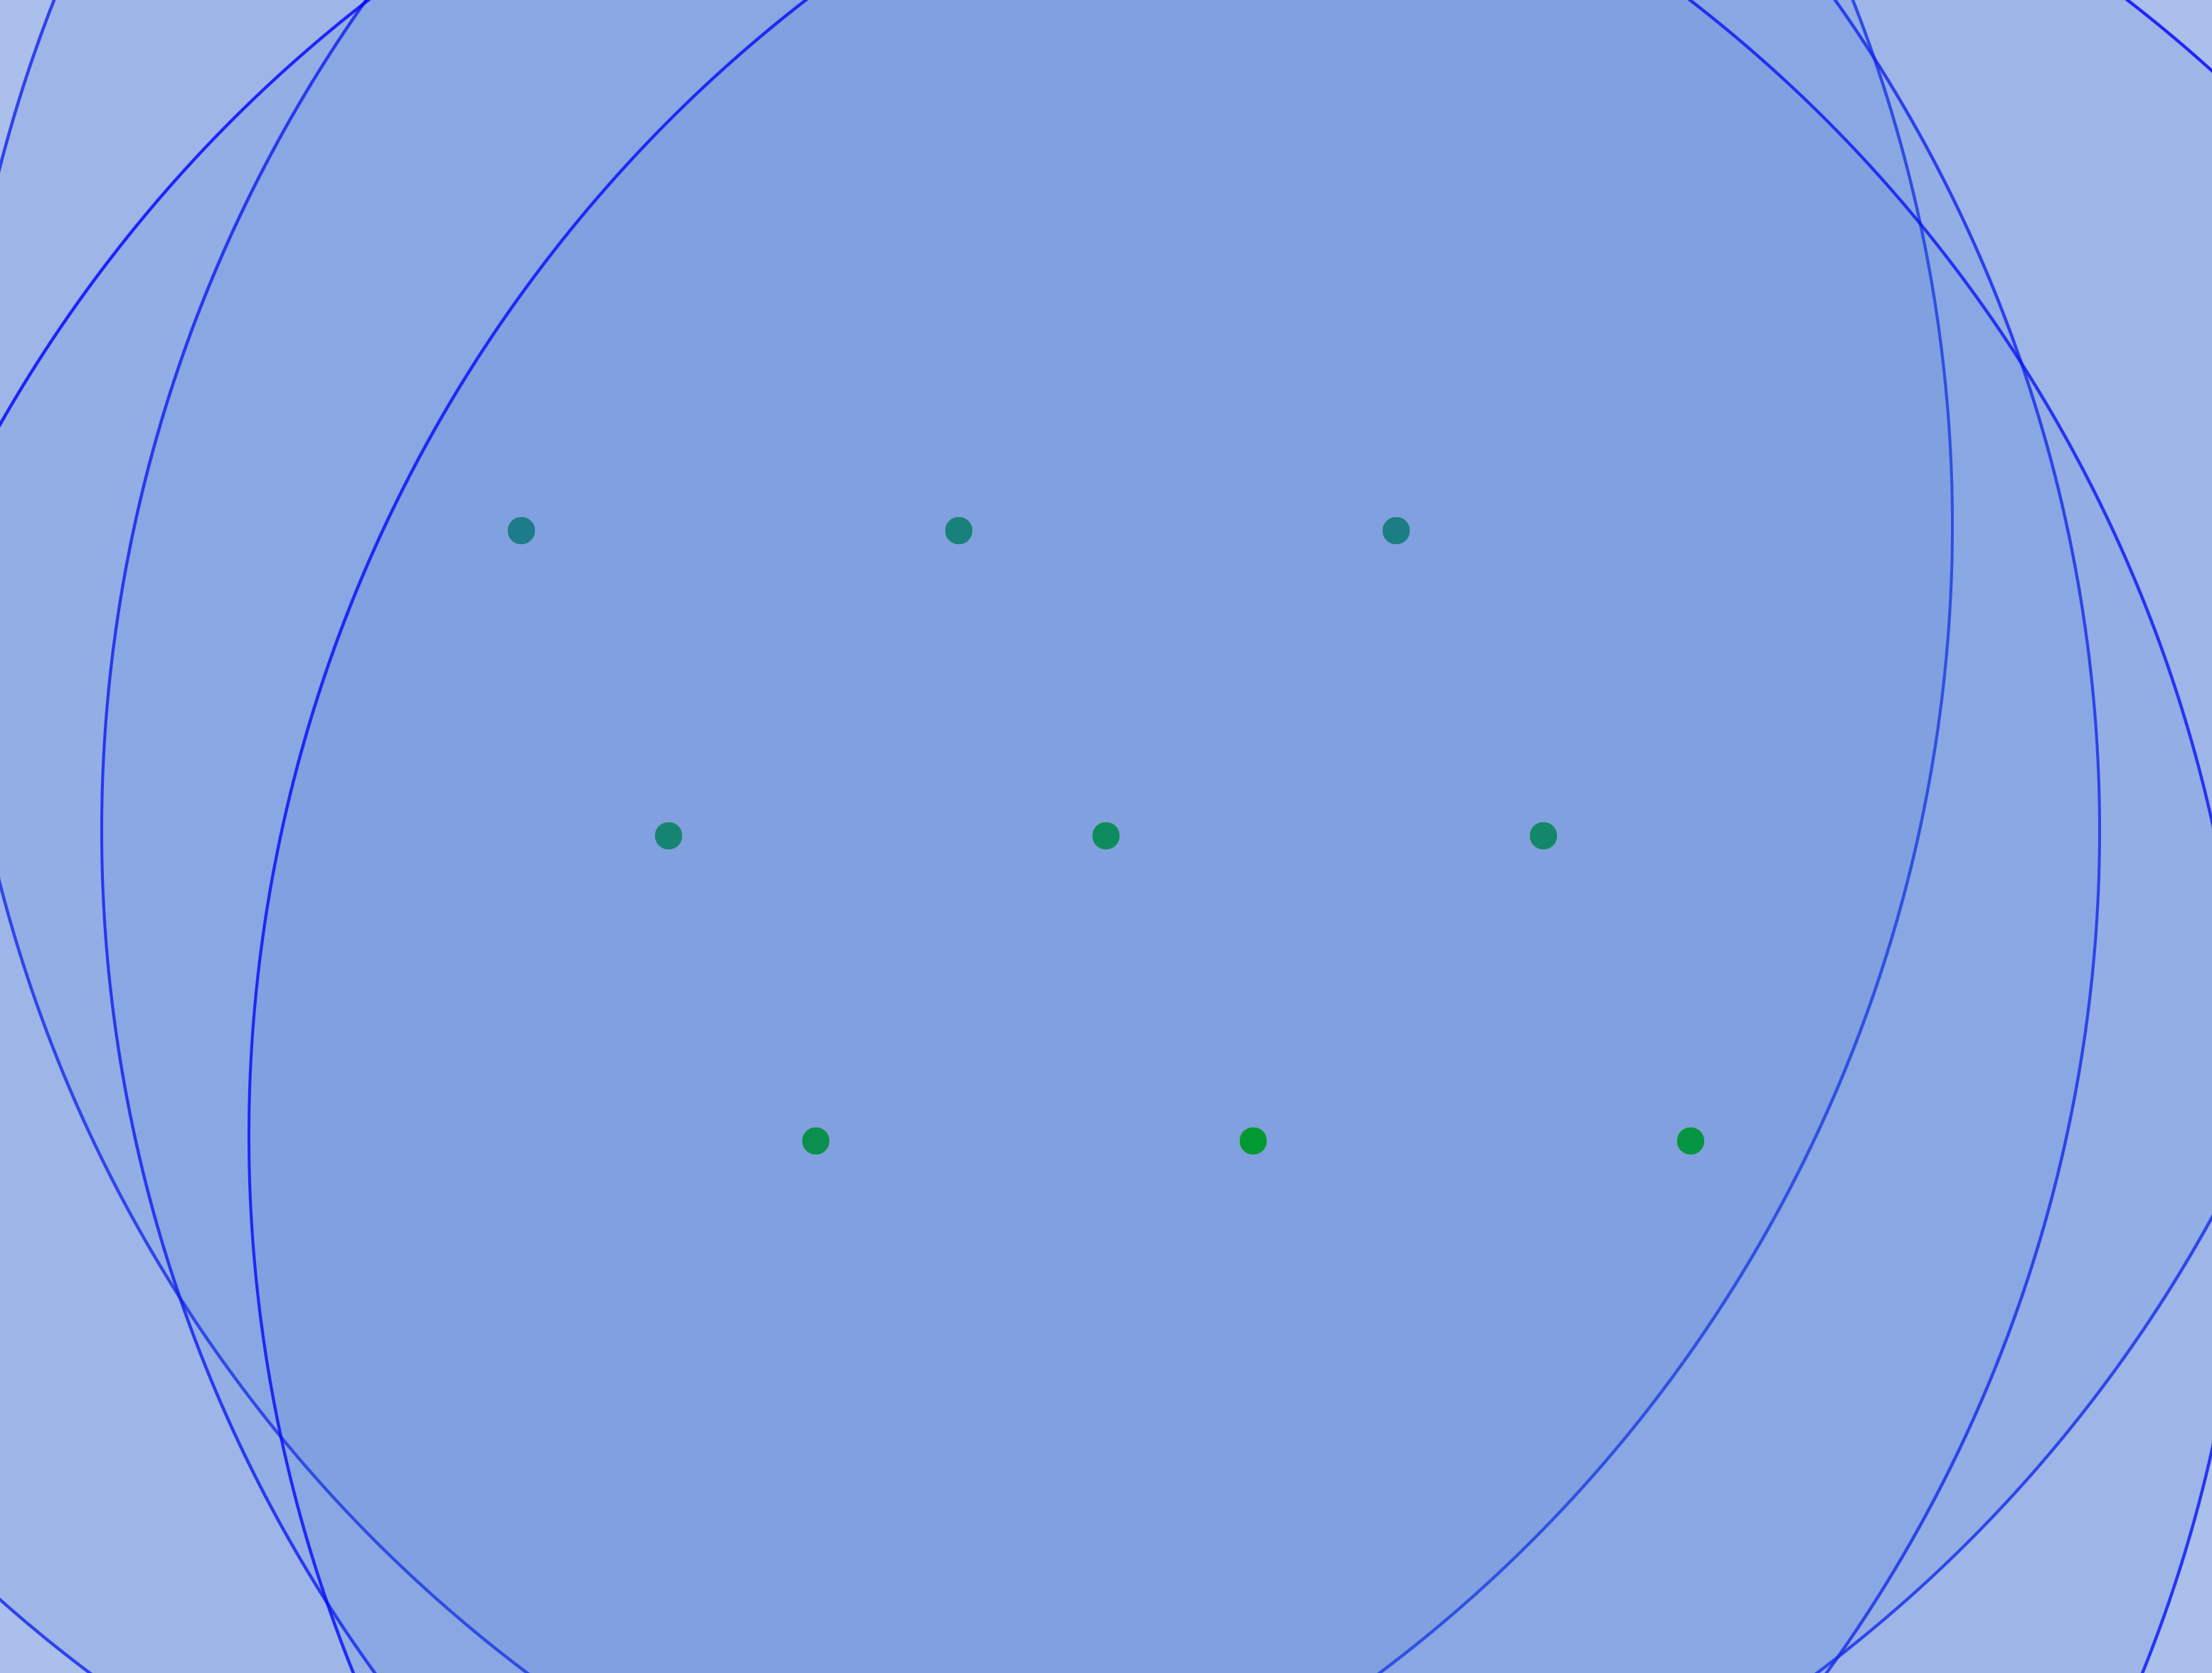
\includegraphics[width=0.5\linewidth]{./image/gaussian_3.png}
			\caption{The distribution when $s$ is large enough}%
			\label{fig:gaussian_3}
		\end{figure}
	\end{frame}
	\subsubsection{The Reduction}
			\begin{algorithm}
			\caption{Solving SVP using SIS oracle}
			\label{alg:decision_to_search}
			\begin{algorithmic}
				\FOR{$m$ times}
				\STATE Pick a random lattice point $v_i$
				\STATE Gaussian sample a point $a_i=v_i+r_i$ round to $\mathbb{Z}^n_q$ around $v_i$
				\ENDFOR
				\STATE $\mathbf{A}=(a_1,a_2,...,a_m)\rightarrow$ SIS oracle
				\STATE SIS oracle $\rightarrow \mathbf{z}$ 
				\STATE Output the short lattice vector: $\mathbf{R}\mathbf{z}$
			\end{algorithmic}
		\end{algorithm}
	\section{Learning With Errors Problem (LWE)}
	\subsection{Definition of LWE}
	Consider an additive group $\mathbb{T}=\mathbb{R}/\mathbb{Z}$ which is constructed modulo one. For error, produce a fixed probability distribution over $\mathbb{T}$ denoted as $\varphi$. 
	
	We than define a distribution over $\mathbb{Z}_q^n\times \mathbb{T}$ as
	\begin{enumerate}
		\item Randomly get a vector $a\in \mathbb{Z}_q^n$ following uniform distribution.
		\item Randomly get a number $\epsilon\in\mathbb{T}$ following distrubtion $\varphi$.
		\item Compute addtion and division under $\mathbb{T}$, inner product in $\mathbb{Z}_q^n$ calculate $t=<a,s>/q+e$.
		\item Pair $(a,t)$ is a sample.
	\end{enumerate}
	Denote the entire sample set as $A_{s,\varphi}$.
	\subsubsection{Search problem}%
	\begin{frame}
		With above definition, we define the LWE search problem as trying to find $s$, given polynomial amout of samples from $A_{s,\varphi}$. Most times we studied a special case of LWE, where $\varphi$ is the nomal distrubtion as origin point with variance of $ \frac{\alpha^2}{2\pi} $, i.e. $e^{-\pi(|x| / \alpha)^{2}}/\alpha$.
	\end{frame}
	\subsubsection{Decision problem}%
	\begin{frame}
		On the other hand, LWE decision problem is to tell the difference between a LWE distributed input and a uniformly random input.
	\end{frame}
	\subsection{Average Hardness}%
	\begin{frame}
		Peikert proved that the worst case of LWE can be reducted to GapSVP in polynomial time, considering a approximate output~\cite{hardness_of_lwe}.
	\end{frame}
	\section{Ring learning with errors key exchange}
	\title{algorithm}
		\begin{algorithm}
			\caption{Initiation}
			\label{alg:initiation}
			\begin{algorithmic}
				\STATE $s_{I}$, $e_{I} \gets polynomials\ with\ coefficients\ from\ \chi _{\alpha}\ distribution $
				\STATE $p_{I}\gets as_{I}+2e_{I}$
				\STATE return $p_I$
			\end{algorithmic}
		\end{algorithm}
		
		\begin{algorithm}
			\caption{Response}
			\label{alg:Response}
			\begin{algorithmic}
				\STATE $\mathbf{E}\gets \left\{-\left\lfloor\frac{q}{4}\right\rfloor, \ldots,\left\lfloor\frac{q}{4}\right\rceil\right\} of Z q=\left\{-\frac{q-1}{2}, \ldots, \frac{q-1}{2}\right\}$
				\STATE $s_{R}, e_{R}\gets polynomials\ with\ coefficients\ from\ \chi _{\alpha}\ distribution$
				\STATE $p_{R} \gets as_{R}+2e_{R}$
				\STATE $e'_{R} \gets sample from \chi _{\alpha}\ distribution$
				\STATE $k_{R} \gets p_{I}s_R+2e'_{R}$
				\FOR{each coefficient $k_{R_i}$ of $k_R$}
				\IF{$k_{R_i} \in E$}
				\STATE $w_i \gets 0$
				\ELSE
				\STATE $w_i \gets 1$
				\ENDIF
				\ENDFOR
				\STATE $sk_R = \left(k_R+w \cdot \frac{q-1}{2}\right) \bmod q \bmod 2$
				\STATE return $p_R$, $w$
			\end{algorithmic}
		\end{algorithm}
	\section{Possible Attack for Lattice-based Cryptography}
	\subsection{Fault Attacks}
	\begin{frame}{Fault Attacks}
		Although lattice-based Cryptography is the most safe algorithm, there still exists the implementation level fault, which makes the attack possible. Here we mainly talked about three fault attacks
	\end{frame}
	\begin{frame}{Loop-Abort Faults on Lattice-based Signature}
		in 2018, Espitau proposed a loop-abort faults applied on lattice-based signature.\cite{loopAbortFaults} In this research, they applied two attack but with roughly the same type of faults, so that the attacker could lead to a loop inside the algorithm of the signature and abort early. The first attack is in the Fiat-Shamir family. By inputing a fault in the loop, they could get the commitment value, which is a random polynomial. This could leak enough information for recovering the entire signing key. For the GPV-based hash-and-sign signature scheme, when it is applied into the early loop abort, the original ciphertext will become a linear combination of the parts of the secret lattice. Therefore, in this way, we could recover the key by repeating this process.
	\end{frame}
	\subsection{Effective Attacks}
	\subsubsection{Physical Attack}
	\begin{frame}
		One classical way of attacking the lattice-based schemes is the physical attack, since there are little research results on the physical security of lattice-based cryptography. Moreover, physical attack is easier comparing to other attack. \cite{loopAbortFaults}
	\end{frame}
	\subsubsection{Cryptanalysis of GGH}
	\begin{frame}
		In 2018,Yupu Hu and Huiwen Jia presented several efficient attacks on GGH.\cite{GGH_Map} In the attack testing experiments, the most important part is the specific modular operations so as they could reduce the effect of noise of GGH. In this way, with little lattice-reduction tools, MKE(multipartite key exchange) would be attacked. To break WE(witness encryption), they made use of the hardness of exact-3-call(X3C) problem. By combining these two steps, enough useful information for attack could be gotten and the attack towards GGH succeeds.
	\end{frame}
	\subsubsection{Attack against Cai-cusick}
	\begin{algorithm}
		\caption{\textbf{The Ciphertext-Only Attack}}
		\begin{algorithmic}
			\REQUIRE 
			$v_{\sigma(0)},v_{\sigma(1)},...,v_{\sigma(m)}$: The public key\\
			$b$: the maximum of the public key\\
			$C$: the ciphertext\\
			\ENSURE
			$M=(a_0,a_1,...,a_m)$: The corresponding message\\
			"Failure": message corresponding to errors\\
			\STATE Use public keys to compute the Gram-Schmidt orthogonalization vectors:$v_{\sigma(0)}^\ast,v_{\sigma(1)}^\ast,...,v_{\sigma(m)}^\ast$
			\IF{$min_{0\leq i\leq m}\parallel v_{\sigma(i)}^\ast\leq b\rightarrow $"Failure"}
			\STATE halt
			{$3-8$}
			\ENDIF
			\STATE $i:=m$
			\REPEAT
			\STATE $a_i:=\left[\frac{<v_{\sigma_{(i)}}^\ast,C>}{\parallel v_{\sigma_{(i)}}^\ast\parallel^2} \right]$
			\STATE $C:=C-a_iv_{\sigma_{(i)}},i:=i-1$
			\UNTIL{$i<0$}
			\RETURN $(a_0,a_1,...,a_m)$
		\end{algorithmic}	
	\end{algorithm}
\section*{reference}
\begin{frame}
	\printbibliography
\end{frame}
\end{document}